\documentclass[a4paper]{article}

\usepackage[english]{babel}
\usepackage{xspace}
\usepackage{amsmath, amsthm, amssymb, mathrsfs, dsfont}
\usepackage{graphicx}
\usepackage[all]{xy}
\usepackage{bussproofs}
\usepackage{graphicx,float,wrapfig}

\usepackage{amssymb}
\usepackage{latexsym}
\usepackage{algorithm}
\usepackage[noend]{algpseudocode}
\usepackage{hyperref} 
\usepackage{float}

\usepackage{subfigure}

\usepackage[backend=bibtex]{biblatex}

% Default fixed font does not support bold face
\DeclareFixedFont{\ttb}{T1}{txtt}{bx}{n}{8} % for bold
\DeclareFixedFont{\ttm}{T1}{txtt}{m}{n}{8}  % for normal

% Custom colors
\usepackage{color}
\definecolor{deepblue}{rgb}{0,0,0.5}
\definecolor{deepred}{rgb}{0.6,0,0}
\definecolor{deepgreen}{rgb}{0,0.5,0}

\usepackage{listings}

% Python style for highlighting
\newcommand\pythonstyle{\lstset{
		language=Python,
		basicstyle=\ttm,
		otherkeywords={self},             % Add keywords here
		keywordstyle=\ttb\color{deepblue},
		emph={MyClass,__init__},          % Custom highlighting
		emphstyle=\ttb\color{deepred},    % Custom highlighting style
		stringstyle=\color{deepgreen},
		frame=tb,                         % Any extra options here
		showstringspaces=false            % 
	}}
	
	
	% Python environment
	\lstnewenvironment{python}[1][]
	{
		\pythonstyle
		\lstset{#1}
	}
	{}

\usepackage[utf8]{inputenc}

\def\fCenter{{\mbox{$\, \rightarrow \, $}}}

% Optional to turn on the short abbreviations
\EnableBpAbbreviations

%\newcommand{\url}[1]{\texttt{#1}}
\newcommand{\shellcmd}[1]{\\\indent\indent\texttt{\footnotesize\# #1}\\}

\newcommand*{\QEDA}{\hfill\ensuremath{\blacksquare}}%

\bibliography{bibliography}
%\bibliographystyle{ieeetr}
 

\begin{document}

 \title{\textbf{Algorithmic Decision Theory} \\ Final course evaluation project
 \\  ~\\ \normalsize{deadline Tuesday, June 28, 09:00}}
 \author{Maciej Żurad \\ \url{maciej.zurad@gmail.com}}

\date{}

\maketitle



\section{What is apparently the best decision action in your problem from the environmental point of view, from the economic point of view, from the societal point of view, and from a global multi-objectives compromise point of view ?}

All operations on data were done using \texttt{Digraph3}\footnote{Digraph3 is hosted at \url{https://github.com/rbisdorff/Digraph3}} Python3 package, which implements decision aid algorithms in the context of bipolarly-valued outranking approach.

Let us first take a look, at best decision from the point of view of each category. In order to see that, we have to first make sure to neglect all other criteria. To achieve that, we must first create a partial performance tableau from the original performance tableau. Program \texttt{code/bcr\_categories.py} implements all operations needed to show Best Choice Recommendation from the environmental, economical and societal point of view. The output of this program was also saved to \texttt{code/bcr\_categories.out}

We first find a set of criteria that belong to a certain category (e.g Economical) and create a partial performance tableau with only these criterias. We now create a Bipolar Outranking Digraph from that performance table and use Rubis\cite{bisdorff2008r, bisdorff2006choices} solver to get a potential Best Choice Recommendation, which is depicted in Figure \ref{lst:rubis}.

\begin{figure}[H]
\begin{center}
\begin{python}
from perfTabs import *
from outrankingDigraphs import BipolarOutrankingDigraph
pt = XMCDA2PerformanceTableau('project_2')
criterias = [c for c, val in pt.criteria.items() if 'Eco' in val['name']]
ppt = PartialPerformanceTableau(pt,criteriaSubset=criterias)
partial_digraph = BipolarOutrankingDigraph(ppt)
partial_digraph.showRubisBestChoiceRecommendation()
\end{python}
\end{center}
\caption{Rubis Best Choice Recommendation code-snippet}
\label{lst:rubis}
\end{figure}

Outranking Digraph is based on the idea of outranking. For two alternative $a$ and $b$, $a$ outranks $b$ $(a S b)$ if there exist a significant majority of criteria supporting that $a$ is \emph{at least} as good as $y$ and no considerable counter-performance (\emph{no veto}) is observed on any discordant criterion. For each Outranking Digraph a relation table was generated and saved in directory:

\texttt{report/figures/*\_bipolar\_adj\_matrix.html} 

\subsection{From the Economical point of view}

The output of the Rubis Best Choice Recommendation from the Economic point of view is the following: we get three potential BCRs, an alternative \textbf{a19} and a tuple of alternatives \textbf{(a31, a48)} with the same values. All the values share the same \emph{dominance} at 33.33 and \emph{absorbency} at -100.00. However, \textbf{a19} is a \textbf{better} candidate, because \emph{covering} is maxed out at 100.00\% and \emph{determinateness} is higher as well at 66.67\% compared to 50.00\%. Another way to confirm that \textbf{a19} is in fact a better BCR candidate is to check the Condorcet and the Weak-Condorcet winners. Figure \ref{lst:condo} is showing us how to calculate this. The Condorcet winner from Economical point of view is as expected \textbf{a19} and the Weak-Condorcet winners are \textbf{a19, a36, a48}, which also disqualifies previously seen \textbf{a31}. Therefore, \textbf{a19} is the best choice from Economical point of view!

\begin{figure}[H]
	\begin{center}
		\begin{python}
weak_condorcet_winners = partial_digraph.weakCondorcetWinners()
condorcet_winners      = partial_digraph.condorcetWinners()
		\end{python}
	\end{center}
	\caption{Condorcet and Weak Condorcet winner code-snippet}
	\label{lst:condo}
\end{figure}



\subsection{From the Environmental point of view}
\label{sec:env}

The output of the Rubis Choice Recommendation from the Environmental point of view is \textbf{a28, a41, a48}, where all alternatives have exactly the same values, when it comes to \emph{irredundancy, independence, dominance, absorbency, covering} and \emph{determinateness}. Condorcet winner from Environmental point of view gives us the same alternatives and the Weak-Condorcet winner gives us the same together with \textbf{a35}. Which leaves us with \textbf{3} Best Choice Recommendation from Environmental point of view: \textbf{a28, a41, a48}.

\subsection{From the Societal point of view}

Rubis Choice Recommendation from the Societal point of view bring the same situation as from Environmental point of view (section \ref*{sec:env}). The Rubis solver gives us three alternatives: \textbf{a18, a38, a49}. They also share exactly the same values and the Condorcet winners are also \textbf{a18, a38, a49}. Weak-Condorcet winners are: \textbf{a18, a38, a49, a12, a33, a45}. Another interesting thing we can try is to do Strictly Best Choice by computing the \textbf{codual} of the Outranking Digraph, that is a converse of a dual and after that run this graph through Rubis solver, which is presented in Figure \ref{lst:strict}. This gives a single BCR\footnote{BCR stands for Best Choice Recommendation} which is a list and contains all Weak-Condorcet winners. However, when we look into the characteristic vector, which represents, whether an alternative may indeed be considered a best choice, we see that only Condorcet winners are determined and that sole Weak-Condorcet winners are not relevant, because they have a 0.0 value. In the end I chose only those 3: \textbf{a18, a38, a49} to be the BCRs from Societal point of view. 

\begin{figure}[H]
	\begin{center}
		\begin{python}
codual_partial = ~(-partial_digraph)                  # computes codual
codual_partial.showRubisBestChoiceRecommendation()
		\end{python}
	\end{center}
	\caption{Codual of the Outranking Digraph and Strict Best Choice}
	\label{lst:strict}
\end{figure}

\subsection{From the global multi-objectives compromise point of view}
\label{sec:global}

We follow like in the previous examples, except that now we don't have first create Partial Performance Tableau like shown in Figure \ref*{lst:rubis} and we directly call Rubis solver with the the Performance Tableau received when loading the data. We receive following: \textbf{a45, a20} and a tuple \textbf{(a38, a48)}. The Condorcet winners are also \textbf{a45, a20} and as we would expect the Weak-Condorcet winners are \textbf{a45, a20, a38, a48}. Figure \ref{fig:20and45} presents the values for alternatives \textbf{a20, a45} and figure \ref{fig:38_48} presents for \textbf{(a38, a48)}. We can see that \textbf{a45} has the best values, not only it has the highest \emph{determinateness} but also \emph{dominance}, which makes it the \texttt{Best Choice Recommendation} from the global multi-objectives compromise point of view.

\begin{figure}[H]
	\hfill
	\subfigure[Alternative 20]{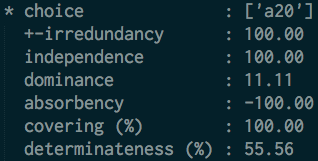
\includegraphics[width=5cm]{figures/full_20}}
	\hfill
	\subfigure[Alternative 45]{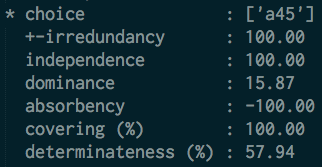
\includegraphics[width=5cm]{figures/full_45}}
	\hfill
	\caption{BCR candidates - \textbf{a20} and \textbf{a45}}
	\label{fig:20and45}
\end{figure}

\begin{figure}[H]
	\centering
	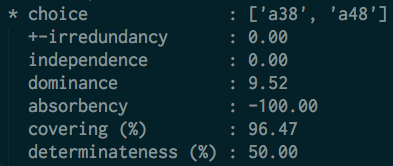
\includegraphics[width=5cm]{figures/full_38_48}
	\caption{BCR candidates - \textbf{a38} and \textbf{a48}}
	\label{fig:38_48}
\end{figure}

All the output to calculate BCR from the global multi-objective compromise point of view was saved \texttt{code/bcr\_multi\_objective.out} and can be generated again using \texttt{code/bcr\_multi\_objective.py}.

\section{What are the five potential best compromise choice candidates in your problem ?}
\label{sec:two}

Section \ref{sec:global} described BCR from the multi-objective point of view. We saw there, 4 Best Choice Recommendations that Rubis solver offered, from which I chose a single one (\textbf{a45}). To choose 5, we can now simply choose those 4 and we will be missing only last. To find the $5^{th}$, we will use a performance heatmap, presented in figure \ref{fig:heatmap}. We can generate this performance heatmap very easily. Instead of showing it in browser, I directly save it on a disk using this code snippet depicted in Figure \ref{lst:html}. This heatmap is by default ranked with a Copeland ranking rule, which will be described later on (section \ref{sec:copeland}). If we took 4 BCRs that we defined previously from the Heatmap, then we would take from row 1,2,3 and 6. A common sense would tell us to take the next best in this ranking, which would be in row 4 (\textbf{a35}). We will see later that a different ranking rule would give us a different result. Therefore, the five potential best compromise choice candidates are \textbf{a45, a20, a38, a48} and \textbf{a35}.
\begin{figure}[H]
	\begin{center}
		\begin{python}
def fwrite(string, file):
  with open(file, 'w') as f:
    f.write(string)
    
make_path = lambda x: os.path.join('..', 'report', 'figures', x.lower())

pt = XMCDA2PerformanceTableau('project_2')
html_heatmap = pt.htmlPerformanceHeatmap()
fwrite(html_heatmap, make_path("full_heatmap.html"))    
		\end{python}
	\end{center}
	\caption{Performance Heatmap generation and saving}
	\label{lst:html}
\end{figure}

\begin{figure}
	\centering
	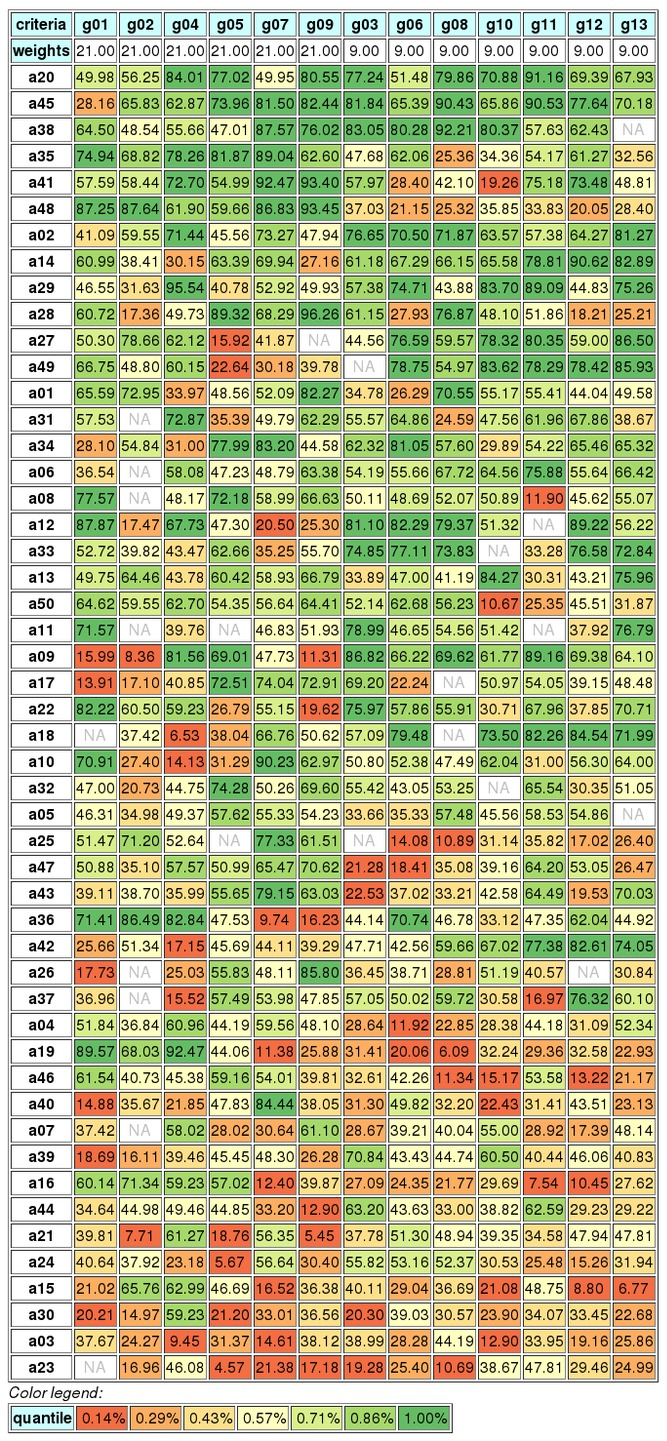
\includegraphics[width=11cm]{figures/full_heatmap}
	\caption{Performance Heatmap with Copeland ranking rule}
	\label{fig:heatmap}
\end{figure}


\section{How would you rank your set of alternatives?}

Ranking is a very tricky process. That is because an Outranking Digraph does not usually present a linear ordering. Pairwise relations do not posses transitive relation. That's because an alternative $a$ can outrank alternative $b$ and also $b$ can outrank $c$. However, that does not imply that an alternative $a$ would \textbf{outrank} $c$. To see, how much of a transitivity is preserved in an outranking digraph, we can calculate Transitivity Degree metric, which is the ratio of outranking arcs over the number of transitive closure arcs in digraph $g$. We can see that if this value is less than 1.0, than we have a digraph that does have some non-transitive relations, which will not be a rare case.

Another problem to correctly rank is the existence of cycles inside a digraph. For instance, if alternative $a$ outranks $b$ and consequently $b$ outranks $c$ and then $c$ outranks $a$, then we have a cycle. Any potential linear ordering of these 3 alternatives will contradict itself. Figure \ref{lst:cycles} presents a code-snippet to calculate Transitivity Degree as well as number of cycles. In my case, the Transitivity Degree was \textbf{0.6012} and \textbf{33} cycles were detected.

The python script with all the code used in this section is called  \texttt{code/ranking\\\_and\_sorting.py} and the output was saved to \texttt{code/ranking\_and\_sorting.out}

In order to deal with these problems, several heuristic have been developed and we will take a look at them.

\begin{figure}[H]
	\begin{center}
		\begin{python}
from perfTabs import *
from outrankingDigraphs import BipolarOutrankingDigraph
pt = XMCDA2PerformanceTableau('project_2')
full_digraph = BipolarOutrankingDigraph(pt)
full_digraph.computeTransitivityDegree()
full_digraph.computeChordlessCircuits()
full_digraph.showChordlessCircuits()
		\end{python}
	\end{center}
	\caption{Computing Transitivity Degree and $\#$ of cycles}
	\label{lst:cycles}
\end{figure}


\subsection{Copeland ranking}
\label{sec:copeland} 

Copeland ranking is very intuitive and computes for each alternative a score resulting from difference between its out-degree and in-degree. Figure \ref{lst:copeland} shows how to compute ranking using this rule.

\begin{figure}[H]
	\begin{center}
		\begin{python}
from linearOrders import CopelandOrder
cop = CopelandOrder(full_digraph)
cop.showRanking()
cop_corr = full_digraph.computeOrdinalCorrelation(cop)
print("Fitness of Copeland's ranking: %.3f" % cop_corr['correlation'])
		\end{python}
	\end{center}
	\caption{Computing Copeland ranking and its fitness}
	\label{lst:copeland}
\end{figure}

I received this ranking from Copeland ranking:\\

\textbf{[a20, a45, a38, a35, a41, a48, a02, a14, a29, a28, a27, a49, a01, a31, a34, a06, a08, a12, a33, a13, a50, a11, a09, a17, a22, a18, a10, a32, a05, a25, a47, a43, a36, a42, a26, a37, a04, a19, a46, a40, a07, a39, a16, a44, a21, a24, a15, a30, a03, a23]}\\

and the following fitness value: \textbf{0.868}

\subsection{Net-Flows ranking}

Net-Flows heuristic is using the values given directly by the outranking digraph $g$. For every alternative $a$, we iterate over all other alternatives $b$ and compute sum of differences between the outranking characteristic $r (a S b)$ and $r (b S a)$.

$$ netFlow(x) = \sum_{y \in Y}(r(x\ S\ y) - r(y\ S\ x))$$

\begin{figure}[H]
	\begin{center}
		\begin{python}
from linearOrders import NetFlowsOrder
nf = NetFlowsOrder(full_digraph)
print('Net flow values for each alternative')

for n,va in enumerate(nf.netFlows):
	print("{0} {2} -> {1:.2f}".format(n+1, *va))

nf.showRanking()
nf_corr = full_digraph.computeOrdinalCorrelation(nf)
print("Fitness of Net-flows ranking: %.3f" % nf_corr['correlation'])
		\end{python}
	\end{center}
	\caption{Computing Net-Flows ranking and its fitness}
	\label{lst:netflows}
\end{figure}

\begin{table}[H]
	\centering
	\begin{tabular}{|c|c|c|}
		\hline
		n                   & alternative & netFlow \\ \hline
		1 & a45 & 7141.27 \\ \hline
		2 & a20 & 6511.11 \\ \hline
		3 & a38 & 5971.43 \\ \hline
		4 & a41 & 5415.87 \\ \hline
		5 & a35 & 4933.33 \\ \hline
		6 & a02 & 3650.79 \\ \hline
		7 & a48 & 3604.76 \\ \hline
		8 & a14 & 3509.52 \\ \hline
		9 & a29 & 3246.03 \\ \hline
		10 & a27 & 3068.25 \\ \hline
		... & ... & ... \\ \hline
	\end{tabular}
	\caption{NetFlows ranking with the netFlow values for the first top 10 alternatives}
	\label{fig:netflows2}
\end{table}

I got the following ranking using Net-Flows heuristic:\\

\textbf{[a45, a20, a38, a41, a35, a02, a48, a14, a29, a27, a49, a28, a34, a33, a09, a01, a06, a12, a13, a31, a18, a11, a50, a08, a17, a10, a22, a32, a05, a47, a42, a43, a36, a25, a26, a04, a37, a40, a46, a07, a19, a39, a44, a21, a16, a24, a30, a15, a23, a03]}\\

and the following fitness value: \textbf{0.877}

\subsection{Kohler's ranking}

Kohler's ranking is also known as \textbf{ranking-by-choosing}. The algorithm is fairly easy and can be described in few steps. Step 1, we take the Relation Table from the outranking graph (basically the previously described adjacency matrix). Step 2, for each row, we find it's minimum and we select a row, where this minimum is maximum among other rows. Step 3, we place this alternative at rank highest possible rank. Step 4, we delete corresponding row and column of the last alternative and we go to Step 1 unless table is empty.

\begin{figure}[H]
	\begin{center}
		\begin{python}
from linearOrders import KohlerOrder
ko = KohlerOrder(full_digraph)
ko.showRanking()
ko_corr = full_digraph.computeOrdinalCorrelation(ko)
print("Fitness of Kohler's ranking: %.3f" % ko_corr['correlation'])
		\end{python}
	\end{center}
	\caption{Computing Kohler's ranking and its fitness}
	\label{lst:kohler}
\end{figure}

I received this ranking from Kohler's ranking:\\

\textbf{[a45, a20, a41, a48, a38, a35, a02, a29, a14, a08, a01, a49, a33, a27, a28, a06, a11, a34, a10, a32, a17, a31, a09, a50, a05, a43, a47, a13, a42, a19, a18, a26, a12, a22, a36, a25, a37, a04, a46, a21, a07, a40, a16, a39, a44, a24, a15, a03, a30, a23]}\\

and the following fitness value: \textbf{0.863}

\subsection{Tideman's Ranked-Pairs}

Ranked-Pairs is based on a construction, which incrementally constructs a linear order simultaneously avoiding any cycles on the fly.

\begin{figure}[H]
	\begin{center}
		\begin{python}
from linearOrders import RankedPairsOrder
rp = RankedPairsOrder(full_digraph)
rp.showRanking()
rp_corr = full_digraph.computeOrdinalCorrelation(rp)
print("Fitness of Tideman's Ranked-Pairs rule ranking: %.3f" % rp_corr['correlation'])

		\end{python}
	\end{center}
	\caption{Computing Tideman's Ranked-Pairs ranking and its fitness}
	\label{lst:tideman}
\end{figure}


I received the following ranking from Tideman's Ranked-Pairs:\\

\textbf{[a45, a20, a41, a38, a35, a48, a02, a29, a49, a34, a14, a12, a27, a06, a31, a18, a28, a17, a01, a09, a08, a22, a50, a13, a11, a33, a10, a25, a47, a32, a05, a26, a36, a42, a43, a04, a19, a37, a21, a07, a40, a16, a46, a39, a44, a24, a15, a03, a30, a23]}\\

and the following fitness value: \textbf{0.893}

\subsection{Conclusions on Ranking}

As we can see different Ranking methods give us quite different results. They also have higher or lower fitness values. Highest fitness values was achieved by Tideman's Ranked-Pairs ranking with value 0.893, shortly after that we have Net-Flows ranking with value 0.877 and at the end we have Copeland's with 0.868 and Kohler's with 0.863.

Another important thing is to remember that Copeland and Net-Flows are very fast algorithms, where Kohler's and Tideman's are slower and do not scale so well. There also exist optimal ranking algorithms such as Kemeny and Slater. However, these two algorithms are exponential in complexity and running them on a graph bigger than 15 seems infeasible.

In the end my final ranking is Tideman's ranking, because it exhibited the highest fitness value.

\section{How would you sort your alternatives into performance deciles ? }

In order to sort our alternatives into performance deciles, we have to use Sorting Digraphs. QuantilesSortingDigraphs are subclass of SortingDigraphs, that work well for large graphs. Figure \ref{lst:sorting} shows code-snippet, which allows to compute that. Figure \ref{fig:sorting_graph} presents our graph. The graph shows only 8 rows, because 2 deciles are empty. There is no alternative, which is in the top and bottom deciles ([0.9 - 1.0] and [ 0.0 - 0.1]). Output of the program described in figure \ref{lst:sorting} was saved as well to \texttt{code/ranking\_and\_sorting.out}. From the graph, we can clearly recognize our BCRs candidates and Condorcet winners, which as we would expect are in the top row, together with the $5^{th}$ BCR that we added in section \ref{sec:two}

\begin{figure}[H]
	\begin{center}
		\begin{python}
from sortingDigraphs import QuantilesSortingDigraph
qs = QuantilesSortingDigraph(pt,limitingQuantiles=10)
qs.showSorting()
qs.showQuantileOrdering()
qs.exportGraphViz(make_path("sorted_deciles_graph"))
		\end{python}
	\end{center}
	\caption{Computing Quantile Ordering for 10 quantiles (deciles)}
	\label{lst:sorting}
\end{figure}

\begin{figure}[H]
	\centering
	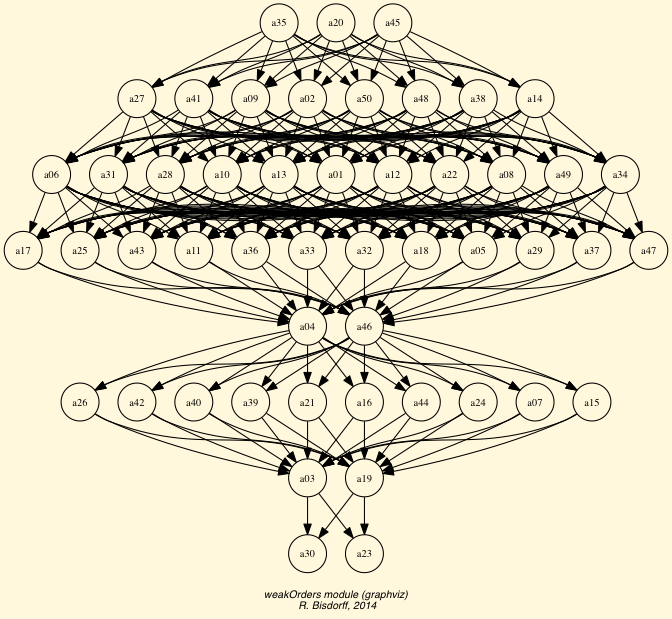
\includegraphics[width=11cm]{figures/sorted_deciles_graph}
	\caption{Decile Sorting Digraph}
	\label{fig:sorting_graph}
\end{figure}



\printbibliography

\end{document} 